
%% bare_conf.tex
%% V1.4b
%% 2015/08/26
%% by Michael Shell
%% See:
%% http://www.michaelshell.org/
%% for current contact information.
%%
%% This is a skeleton file demonstrating the use of IEEEtran.cls
%% (requires IEEEtran.cls version 1.8b or later) with an IEEE
%% conference paper.
%%
%% Support sites:
%% http://www.michaelshell.org/tex/ieeetran/
%% http://www.ctan.org/pkg/ieeetran
%% and
%% http://www.ieee.org/

%%*************************************************************************
%% Legal Notice:
%% This code is offered as-is without any warranty either expressed or
%% implied; without even the implied warranty of MERCHANTABILITY or
%% FITNESS FOR A PARTICULAR PURPOSE! 
%% User assumes all risk.
%% In no event shall the IEEE or any contributor to this code be liable for
%% any damages or losses, including, but not limited to, incidental,
%% consequential, or any other damages, resulting from the use or misuse
%% of any information contained here.
%%
%% All comments are the opinions of their respective authors and are not
%% necessarily endorsed by the IEEE.
%%
%% This work is distributed under the LaTeX Project Public License (LPPL)
%% ( http://www.latex-project.org/ ) version 1.3, and may be freely used,
%% distributed and modified. A copy of the LPPL, version 1.3, is included
%% in the base LaTeX documentation of all distributions of LaTeX released
%% 2003/12/01 or later.
%% Retain all contribution notices and credits.
%% ** Modified files should be clearly indicated as such, including  **
%% ** renaming them and changing author support contact information. **
%%*************************************************************************


% *** Authors should verify (and, if needed, correct) their LaTeX system  ***
% *** with the testflow diagnostic prior to trusting their LaTeX platform ***
% *** with production work. The IEEE's font choices and paper sizes can   ***
% *** trigger bugs that do not appear when using other class files.       ***                          ***
% The testflow support page is at:
% http://www.michaelshell.org/tex/testflow/



\documentclass[conference]{IEEEtran}
% Some Computer Society conferences also require the compsoc mode option,
% but others use the standard conference format.
%
% If IEEEtran.cls has not been installed into the LaTeX system files,
% manually specify the path to it like:
% \documentclass[conference]{../sty/IEEEtran}





% Some very useful LaTeX packages include:
% (uncomment the ones you want to load)


% *** MISC UTILITY PACKAGES ***
%
%\usepackage{ifpdf}
% Heiko Oberdiek's ifpdf.sty is very useful if you need conditional
% compilation based on whether the output is pdf or dvi.
% usage:
% \ifpdf
%   % pdf code
% \else
%   % dvi code
% \fi
% The latest version of ifpdf.sty can be obtained from:
% http://www.ctan.org/pkg/ifpdf
% Also, note that IEEEtran.cls V1.7 and later provides a builtin
% \ifCLASSINFOpdf conditional that works the same way.
% When switching from latex to pdflatex and vice-versa, the compiler may
% have to be run twice to clear warning/error messages.






% *** CITATION PACKAGES ***
%
%\usepackage{cite}
% cite.sty was written by Donald Arseneau
% V1.6 and later of IEEEtran pre-defines the format of the cite.sty package
% \cite{} output to follow that of the IEEE. Loading the cite package will
% result in citation numbers being automatically sorted and properly
% "compressed/ranged". e.g., [1], [9], [2], [7], [5], [6] without using
% cite.sty will become [1], [2], [5]--[7], [9] using cite.sty. cite.sty's
% \cite will automatically add leading space, if needed. Use cite.sty's
% noadjust option (cite.sty V3.8 and later) if you want to turn this off
% such as if a citation ever needs to be enclosed in parenthesis.
% cite.sty is already installed on most LaTeX systems. Be sure and use
% version 5.0 (2009-03-20) and later if using hyperref.sty.
% The latest version can be obtained at:
% http://www.ctan.org/pkg/cite
% The documentation is contained in the cite.sty file itself.






% *** GRAPHICS RELATED PACKAGES ***
%
\ifCLASSINFOpdf
  % \usepackage[pdftex]{graphicx}
  % declare the path(s) where your graphic files are
  % \graphicspath{{../pdf/}{../jpeg/}}
  % and their extensions so you won't have to specify these with
  % every instance of \includegraphics
  % \DeclareGraphicsExtensions{.pdf,.jpeg,.png}
\else
  % or other class option (dvipsone, dvipdf, if not using dvips). graphicx
  % will default to the driver specified in the system graphics.cfg if no
  % driver is specified.
  % \usepackage[dvips]{graphicx}
  % declare the path(s) where your graphic files are
  % \graphicspath{{../eps/}}
  % and their extensions so you won't have to specify these with
  % every instance of \includegraphics
  % \DeclareGraphicsExtensions{.eps}
\fi
% graphicx was written by David Carlisle and Sebastian Rahtz. It is
% required if you want graphics, photos, etc. graphicx.sty is already
% installed on most LaTeX systems. The latest version and documentation
% can be obtained at: 
% http://www.ctan.org/pkg/graphicx
% Another good source of documentation is "Using Imported Graphics in
% LaTeX2e" by Keith Reckdahl which can be found at:
% http://www.ctan.org/pkg/epslatex
%
% latex, and pdflatex in dvi mode, support graphics in encapsulated
% postscript (.eps) format. pdflatex in pdf mode supports graphics
% in .pdf, .jpeg, .png and .mps (metapost) formats. Users should ensure
% that all non-photo figures use a vector format (.eps, .pdf, .mps) and
% not a bitmapped formats (.jpeg, .png). The IEEE frowns on bitmapped formats
% which can result in "jaggedy"/blurry rendering of lines and letters as
% well as large increases in file sizes.
%
% You can find documentation about the pdfTeX application at:
% http://www.tug.org/applications/pdftex





% *** MATH PACKAGES ***
%
%\usepackage{amsmath}
% A popular package from the American Mathematical Society that provides
% many useful and powerful commands for dealing with mathematics.
%
% Note that the amsmath package sets \interdisplaylinepenalty to 10000
% thus preventing page breaks from occurring within multiline equations. Use:
%\interdisplaylinepenalty=2500
% after loading amsmath to restore such page breaks as IEEEtran.cls normally
% does. amsmath.sty is already installed on most LaTeX systems. The latest
% version and documentation can be obtained at:
% http://www.ctan.org/pkg/amsmath





% *** SPECIALIZED LIST PACKAGES ***
%
%\usepackage{algorithmic}
% algorithmic.sty was written by Peter Williams and Rogerio Brito.
% This package provides an algorithmic environment fo describing algorithms.
% You can use the algorithmic environment in-text or within a figure
% environment to provide for a floating algorithm. Do NOT use the algorithm
% floating environment provided by algorithm.sty (by the same authors) or
% algorithm2e.sty (by Christophe Fiorio) as the IEEE does not use dedicated
% algorithm float types and packages that provide these will not provide
% correct IEEE style captions. The latest version and documentation of
% algorithmic.sty can be obtained at:
% http://www.ctan.org/pkg/algorithms
% Also of interest may be the (relatively newer and more customizable)
% algorithmicx.sty package by Szasz Janos:
% http://www.ctan.org/pkg/algorithmicx




% *** ALIGNMENT PACKAGES ***
%
%\usepackage{array}
% Frank Mittelbach's and David Carlisle's array.sty patches and improves
% the standard LaTeX2e array and tabular environments to provide better
% appearance and additional user controls. As the default LaTeX2e table
% generation code is lacking to the point of almost being broken with
% respect to the quality of the end results, all users are strongly
% advised to use an enhanced (at the very least that provided by array.sty)
% set of table tools. array.sty is already installed on most systems. The
% latest version and documentation can be obtained at:
% http://www.ctan.org/pkg/array


% IEEEtran contains the IEEEeqnarray family of commands that can be used to
% generate multiline equations as well as matrices, tables, etc., of high
% quality.




% *** SUBFIGURE PACKAGES ***
%\ifCLASSOPTIONcompsoc
%  \usepackage[caption=false,font=normalsize,labelfont=sf,textfont=sf]{subfig}
%\else
%  \usepackage[caption=false,font=footnotesize]{subfig}
%\fi
% subfig.sty, written by Steven Douglas Cochran, is the modern replacement
% for subfigure.sty, the latter of which is no longer maintained and is
% incompatible with some LaTeX packages including fixltx2e. However,
% subfig.sty requires and automatically loads Axel Sommerfeldt's caption.sty
% which will override IEEEtran.cls' handling of captions and this will result
% in non-IEEE style figure/table captions. To prevent this problem, be sure
% and invoke subfig.sty's "caption=false" package option (available since
% subfig.sty version 1.3, 2005/06/28) as this is will preserve IEEEtran.cls
% handling of captions.
% Note that the Computer Society format requires a larger sans serif font
% than the serif footnote size font used in traditional IEEE formatting
% and thus the need to invoke different subfig.sty package options depending
% on whether compsoc mode has been enabled.
%
% The latest version and documentation of subfig.sty can be obtained at:
% http://www.ctan.org/pkg/subfig




% *** FLOAT PACKAGES ***
%
%\usepackage{fixltx2e}
% fixltx2e, the successor to the earlier fix2col.sty, was written by
% Frank Mittelbach and David Carlisle. This package corrects a few problems
% in the LaTeX2e kernel, the most notable of which is that in current
% LaTeX2e releases, the ordering of single and double column floats is not
% guaranteed to be preserved. Thus, an unpatched LaTeX2e can allow a
% single column figure to be placed prior to an earlier double column
% figure.
% Be aware that LaTeX2e kernels dated 2015 and later have fixltx2e.sty's
% corrections already built into the system in which case a warning will
% be issued if an attempt is made to load fixltx2e.sty as it is no longer
% needed.
% The latest version and documentation can be found at:
% http://www.ctan.org/pkg/fixltx2e


%\usepackage{stfloats}
% stfloats.sty was written by Sigitas Tolusis. This package gives LaTeX2e
% the ability to do double column floats at the bottom of the page as well
% as the top. (e.g., "\begin{figure*}[!b]" is not normally possible in
% LaTeX2e). It also provides a command:
%\fnbelowfloat
% to enable the placement of footnotes below bottom floats (the standard
% LaTeX2e kernel puts them above bottom floats). This is an invasive package
% which rewrites many portions of the LaTeX2e float routines. It may not work
% with other packages that modify the LaTeX2e float routines. The latest
% version and documentation can be obtained at:
% http://www.ctan.org/pkg/stfloats
% Do not use the stfloats baselinefloat ability as the IEEE does not allow
% \baselineskip to stretch. Authors submitting work to the IEEE should note
% that the IEEE rarely uses double column equations and that authors should try
% to avoid such use. Do not be tempted to use the cuted.sty or midfloat.sty
% packages (also by Sigitas Tolusis) as the IEEE does not format its papers in
% such ways.
% Do not attempt to use stfloats with fixltx2e as they are incompatible.
% Instead, use Morten Hogholm'a dblfloatfix which combines the features
% of both fixltx2e and stfloats:
%
% \usepackage{dblfloatfix}
% The latest version can be found at:
% http://www.ctan.org/pkg/dblfloatfix




% *** PDF, URL AND HYPERLINK PACKAGES ***
%
%\usepackage{url}
% url.sty was written by Donald Arseneau. It provides better support for
% handling and breaking URLs. url.sty is already installed on most LaTeX
% systems. The latest version and documentation can be obtained at:
% http://www.ctan.org/pkg/url
% Basically, \url{my_url_here}.




% *** Do not adjust lengths that control margins, column widths, etc. ***
% *** Do not use packages that alter fonts (such as pslatex).         ***
% There should be no need to do such things with IEEEtran.cls V1.6 and later.
% (Unless specifically asked to do so by the journal or conference you plan
% to submit to, of course. )

\usepackage{tabularx}
\usepackage{lipsum}
\usepackage{blindtext}
\usepackage{graphicx}
\usepackage{url}
\usepackage[usenames,dvipsnames,svgnames,table]{xcolor}


\newcommand{\ck}[1]{\textcolor{red}{#1}}

\newcolumntype{K}[1]{>{\centering\arraybackslash}p{#1}}



% correct bad hyphenation here
\hyphenation{op-tical net-works semi-conduc-tor}


\begin{document}

\title{Old is Still Gold: A Comparison of Cyber and Regular Consumer Fraud in The United States}


% author names and affiliations
%\author{\IEEEauthorblockN{Mohammad Taha Khan and Chris Kanich}
%\IEEEauthorblockA{Department of Computer Science, University of Illinois at Chicago\\taha@cs.uic.edu, ckanich@uic.edu}}

% make the title area
\maketitle

% As a general rule, do not put math, special symbols or citations
% in the abstract
\begin{abstract}

While cybercrime is a relatively recent human invention, fraudulent activity has a much longer history. This paper investigates the differences in fraud reporting and targeting among United States based consumers by comparing fraudulent activity mediated by the Internet, with traditional forms of fraud. We study the difference in fraud trends across time, location, ethnic and socio-economic factors. 
Both categories of frauds experience an overall decrease during the holiday season. Individuals who are victimized via traditional methods are more likely to complain using phone or in-person, while a majority of cyber victims submit fraud complaints online. By evaluating the top frauds in each category, we demonstrate how traditional fraudsters have evolved in their operational methodologies to execute scams on the Internet that were initially perpetrated through traditional means.	





 \ck{ADD QUICK AND EASY CONCLUSIONS HERE}.

\end{abstract}


\section{Introduction}

In the United States, a total of more that 25 million people are victims of frauds per year. \cite{anderson2013consumer}. These deceptive scams are a major cause of economic damages to users, not to mention the added externalities of wasted time and stress. These illicit practices have been a part of the underground economy for a while. Initially individuals were tricked by scam calls, mail or in-person fraudsters, however, the rise of the Internet has provided fraudulent entities with a more streamlined exposure to the overall population. A  survey report from 2014 indicated that 47\% of Americans had been victims of an online identity theft. Another recent report released by the  Federal Trade Commission (FTC) revealed that debt collection, identity theft, and impostor scams contribute towards 56\% of the total frauds complaints in 2015 \cite{ftcpress2016} . With the number of Internet users on the rise, the number of cyber frauds is likely to increase over the next couple of years \cite{perharassment}. To deal with the increasing trend, the Federal Bureau of Investigation (FBI), alongside the FTC, has established a similar complaint portal known as the IC3, for the collection of specifically Internet-based fraudulent practices \cite{fbiic3}. This emerging trend of deceptive practices necessitates their study in order to evaluate and mitigate the harm caused to victims individuals.

This paper evaluates the nature of consumer fraud in the United States. Our work provides a comparison between cyber and traditional, non-cyber frauds. We categorize cyber frauds as all those deceptive practices that victimize users online, while regular ones comprise of frauds that target individuals over the phone, with mail, or in-person. While we understand that cyber frauds are a major focus of today's research, our comparison based approach allows us to better understand how they differ from conventional frauds. It also enables us to independently evaluate trends in regular frauds and to see whether fraudsters are adopting online mechanisms to target more individuals. This combined analysis can enable strategic suggestions to develop better fraud reduction methodologies.

To evaluate fraud trends, we use the FTC's Consumer Sentinel database, a dataset of complaints from the year 2013 and 2014. We also collect demographic information from the US Census Bureau \cite{uscensus}. In addition to data collection, we devise a calibration methodology to identify and separate cyber frauds from non-cyber in the complaint dataset. 

Our work provides three main contributions. First, we evaluate the distinctive trends prevalent in cyber and regular frauds in the dataset. This encompasses their reporting numbers and methods. The nature of frauds which are more common in each specific category and the insights on the fraudsters who carry out these specific deceptive activities. Secondly, we look at ethnic, age, education and employment demographics in each specific category and evaluate if certain individuals are more likely to report crimes. Finally, based on our findings we provide suggestive measures that can be taken into account by regulatory agencies to reduce the overall fraud in the United States.

The rest of the paper is structured as follows, section \ref{related} provides a comprehensive overview of the relevant work. In section \ref{data-cal}, we elaborate features of the datasets used in our analysis along with a description of our calibration methodology. Section \ref{eval} summarizes our findings from the data followed by our suggestions to regulatory agencies in \ref{discussion}. We conclude our work in section \ref{conclusion} and discuss avenues of future research.


\section{Related Work}\label{related}


\begin{table*}[h]
\noindent
\centering
\begin{tabular}{K{0.18\linewidth}|p{0.72\linewidth}}
\hline
\multicolumn{1}{c}{\bfseries Data Field} & \multicolumn{1}{c}{\bfseries Field Description}
\\ 
\hline
\hline
Agency Name & The complaint collection agencies associated with the FTC.\\
\hline
Zip code Information & The zip code of the victim and the fraudulent entity.\\
%This provided us with low level granularity for analysis, however, the latter was only available for a subset of the complaints\\
\hline
Contact Method & The primary channel used by the fraudulent entity to contact the victim e.g. Internet, phone, mail.\\
\hline
Fraud Description & A description of nature the fraud, and its type e.g. credit card, fake product, debt collection.\\
\hline
Fraud \&
 Reporting Date & The dates when the fraud initially occurred and the date on which is was reported.
\\
\hline
\end{tabular}
\vspace{8pt}
\caption{data field descriptions primarily used for data calibration and analysis}\label{ftcdata}
\vspace{-20pt}
\end{table*}

As our work evaluates both cyber as well as regular frauds, we provide related work that encompasses both of these categories. However, we elaborate more on recent research which focuses on cyber frauds as more individuals are victims of these crimes \cite{anderson2013consumer} due to the increased Internet usage trends for sensitive activities. Before the Internet became a primary hub of economic and social activity, researchers measured \cite{clarke2001controlling} and developed techniques based on statistical models \cite{brause1999neural, moreau1997detection, bolton2002statistical, snyder2015no} to detect phone and credit card based frauds. In the past few years,  research evaluations have shifted focus towards cyber activity \cite{ablon2016consumer, piper2002, ionescu2011fraud, howard2007cyber} due to its high rate and the increased potential for harm.

Even though term \emph{"cyber fraud"} is usually associated with Computer Science, its recent socio-economic impact has motivated researchers in Economics, Law, and Finance to explore solutions by incorporating methodologies specific to their areas. Ionescu et. al \cite{ionescu2011fraud} characterize the types and sources cyber frauds in global digital networks, they link the increase of financial fraud to the prevalent usage of Internet services for financial management and transactions. The authors suggest the involvement of all stakeholders and employees through awareness and training for containing and mitigating fraud. Similarly, Howard et. al \cite{howard2007cyber} study malicious code attacks against financial networks and suggest technical detection and mitigation techniques for financial infrastructure. \cite{piper2002} studies how the cyber criminals have several potential advantages over their opposing law enforcement agencies. They suggest some practical steps to even out the differential gap.

Due to an increase in the overall concern for online fraudulent activity, there has also been state-sponsored research that measures the impact of fraud. Smyth et. al \cite{smyth2011measuring} measure the extent of cyber fraud in Canada in 2011. Their work indicates that a major chunk of frauds does not get recorded and suggest a need for a sentinel record fraud data, similar to the FTC complaint center in the US.

Another significant area of research focuses on understanding the demographics of fraud victims. A recent FTC Report \cite{raval2016determines} uses complaint data to quantify complaint rates and across different ethnic and education groups in the US. \cite{garrett2010consumers} also look at how demographics effect the likelihood of an individual to complain about fraud. Researchers in \cite{ablon2016consumer} provide a comprehensive survey report that sums the reactions of the victims of an online data breach. They categorize their results in different income, education, age, and ethnic groups. Such research aims to provide organizations with informed insight to better develop policies for consumer rights protection.

In comparison to previous research which individually look at either cyber of regular fraud, w work provides a unique angle of evaluation. We evaluate characteristics for both types of cyber and regular frauds and their demographic trends.

\section{Data and Calibration} \label{data-cal}

In this section we explain the characteristics of our datasets and the sources they were obtained from. We also provide insight into the essential data processing and calibration methodology that we incorporate to classify and filter the data for a fair evaluation of our questions.

\subsection{Data Description}

\subsubsection{FTC Complaint Dataset}

\begin{table}[h]
\centering
\begin{tabular}{c|c}
\hline
{\bfseries Description} & \multicolumn{1}{c}{\bfseries Value}
\\
\hline
\hline
\% Cyber Complaints &52.1\\
\hline
\% Regular Complaints & 47.9\\
\hline
Month with Most Complaints & July 2013\\
\hline
Month with Least Complaints & Feb 2013\\
\hline
\end{tabular}
\vspace{8pt}
\caption{t-test results for cyber and regular frauds in different periods}\label{ttest}
\vspace{-10pt}
\end{table}


The primary dataset that we use for our evaluation is a corpus of the complaint logs filed at different collections agencies and reported to the FTC during the months Jan 2013 to June 2014. The Dataset is comprised of 865K complaints aggregated for cyber as well as regular fraud instances during the time period. Table \ref{ftcdata} shows the fields of the original dataset along with their description summary. For the purposes of brevity, we only include the fields that were used in our analysis.
\\
\subsubsection{US Census Datasets}
Zip code information in our complaint dataset allows us to perform demographic analysis of the frauds. We obtain the demographic information associated with zip codes available at the US Census Bureau website \cite{uscensus}. The specific information that we collect is stated below:

\begin{itemize}
\vspace{8pt}
  \item Population density per zip code
  \item Education and income data \footnote{We obtained education data was obtained from \cite{zipatlas}.}
  \item Age statistics
  \item Race and ethnic information
  \vspace{8pt}
\end{itemize}

As zip codes provide a low level granularity, to aggregate adjacent zip codes we obtain the Zip codes to the Metropolitan Statistical Area (MSA) mappings from \cite{uslaborstats}. MSA are essentially groups of geographically connected zip codes that demonstrate strong social and economic linkage. While there are more than 40,000 zip codes in the United States there are only 382 distinct MSAs \cite{uscensus}.

\subsection{Calibration Methodology}

As the FTC dataset was aggregated for all fraud channels a major calibration step we perform is to tag each crime complaint as either cyber or regular. An associated challenge for this was our limited view of the fraud description. To perform this calibration we use the \textbf{Contact Method} and \textbf{Fraud Description} fields from Table \ref{ftcdata}. We flag a complaint as cyber if the victims primary contact method was through online media, these are primarily websites, social networks, email and IM. For the remainder of the complaints we look at the description. If the complaint description involves something associated with Internet, we classify it as a cyber fraud regardless of how the victim was initially approached. Figure \ref{classify} provides a depiction of our classification methodology. This process  provides us with two distinct categories  and enables a fair comparison of the frauds. 
     

\begin{figure}[t]
\centering
  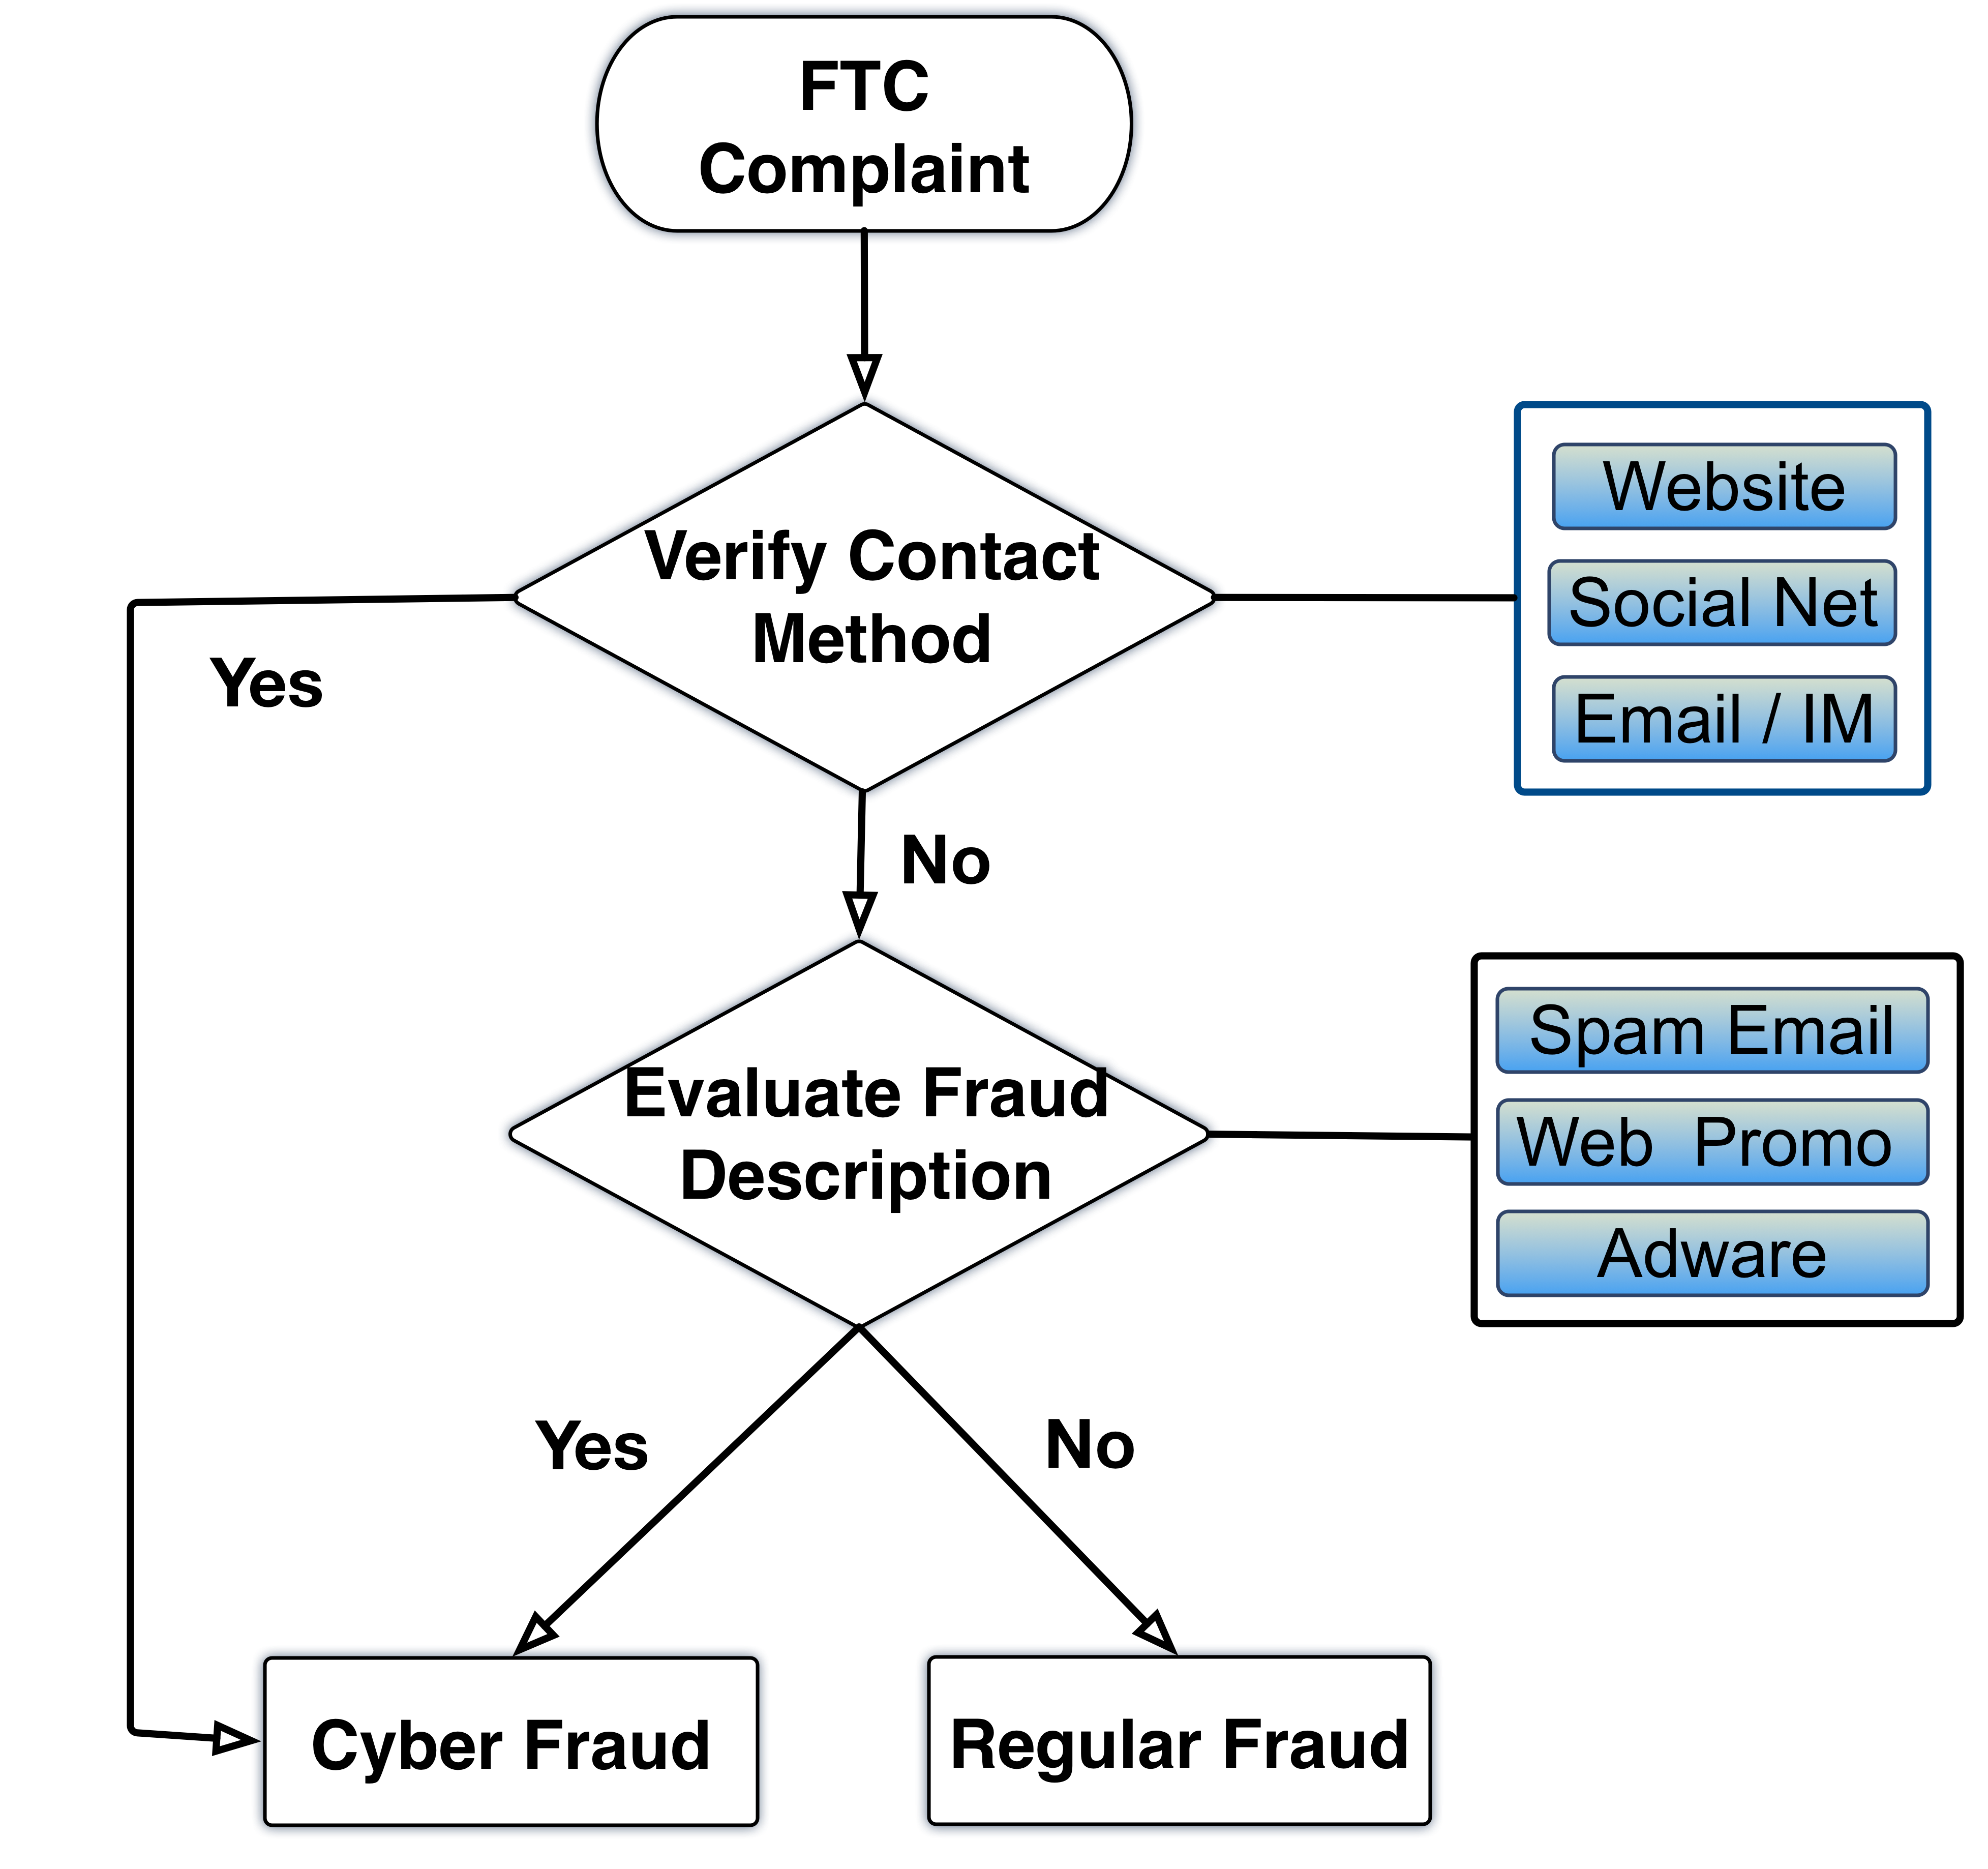
\includegraphics[scale=0.28]{graphics/methodology.png}
  \caption{Classification Methodology for Regular and Cyber Fraud}
  \label{classify}
\end{figure}

\section{Evaluation}\label{eval}

Our evaluation section can be divided into two main components. First, we look at the different aspects and trends within the complaint dataset and elaborate on certain prominent characteristics between regular and cyber frauds. The second part of our evaluation focuses on an in-depth analysis of the demographics linked with the fraud types.



\subsection{Fraud Variation over Time}

\begin{table}[b]
\centering
\begin{tabular}{cc}
\hline
\multicolumn{1}{c}{\bfseries Fraud Type} & \multicolumn{1}{c}{\bfseries \emph{p-value}
Coefficient}
\\
\hline
\hline
Cyber & 0.014\\
\hline
Regular & 0.003\\
\hline
\end{tabular}
\vspace{8pt}
\caption{t-test results for cyber and regular frauds in different periods}\label{ttest}
\vspace{-10pt}
\end{table}

We initially perform a temporal analysis of the 15-month dataset to evaluate how the fraud reporting varies, over time and explore when a certain fraud is more likely to be reported. As a limitation of our dataset\footnote{The dataset had significant missing values for the date if initial contact of fraud, Figure \ref{reportingfig} (a) shows that approximately 70\% of reporting dates were within a week of the date when the incident occurred.}, we use the reporting date as an estimate of fraud count for a specific date. While the overall rate of fraud remains consistent, we observe significant variations in the winter holiday season. To investigate this, we select two distinct, 20 day periods in the dataset; we label them as \textbf{Working} (Aug, 15  to Sept, 5) and \textbf{Holiday} (Dec 15, to Jan, 5). Figure \ref{temporal} shows the variation of cyber and regular frauds within the two specific time periods. We observe a significant drop in the frauds during the the holiday time period. Individually, cyber fraud decreases by 26\% while  regular fraud decreases by a much larger value of 56\%. We believe that the larger decrease in regular frauds is an overestimate as result of a bias that we explain using additional findings from the next section.

\begin{figure}[t]
\centering
  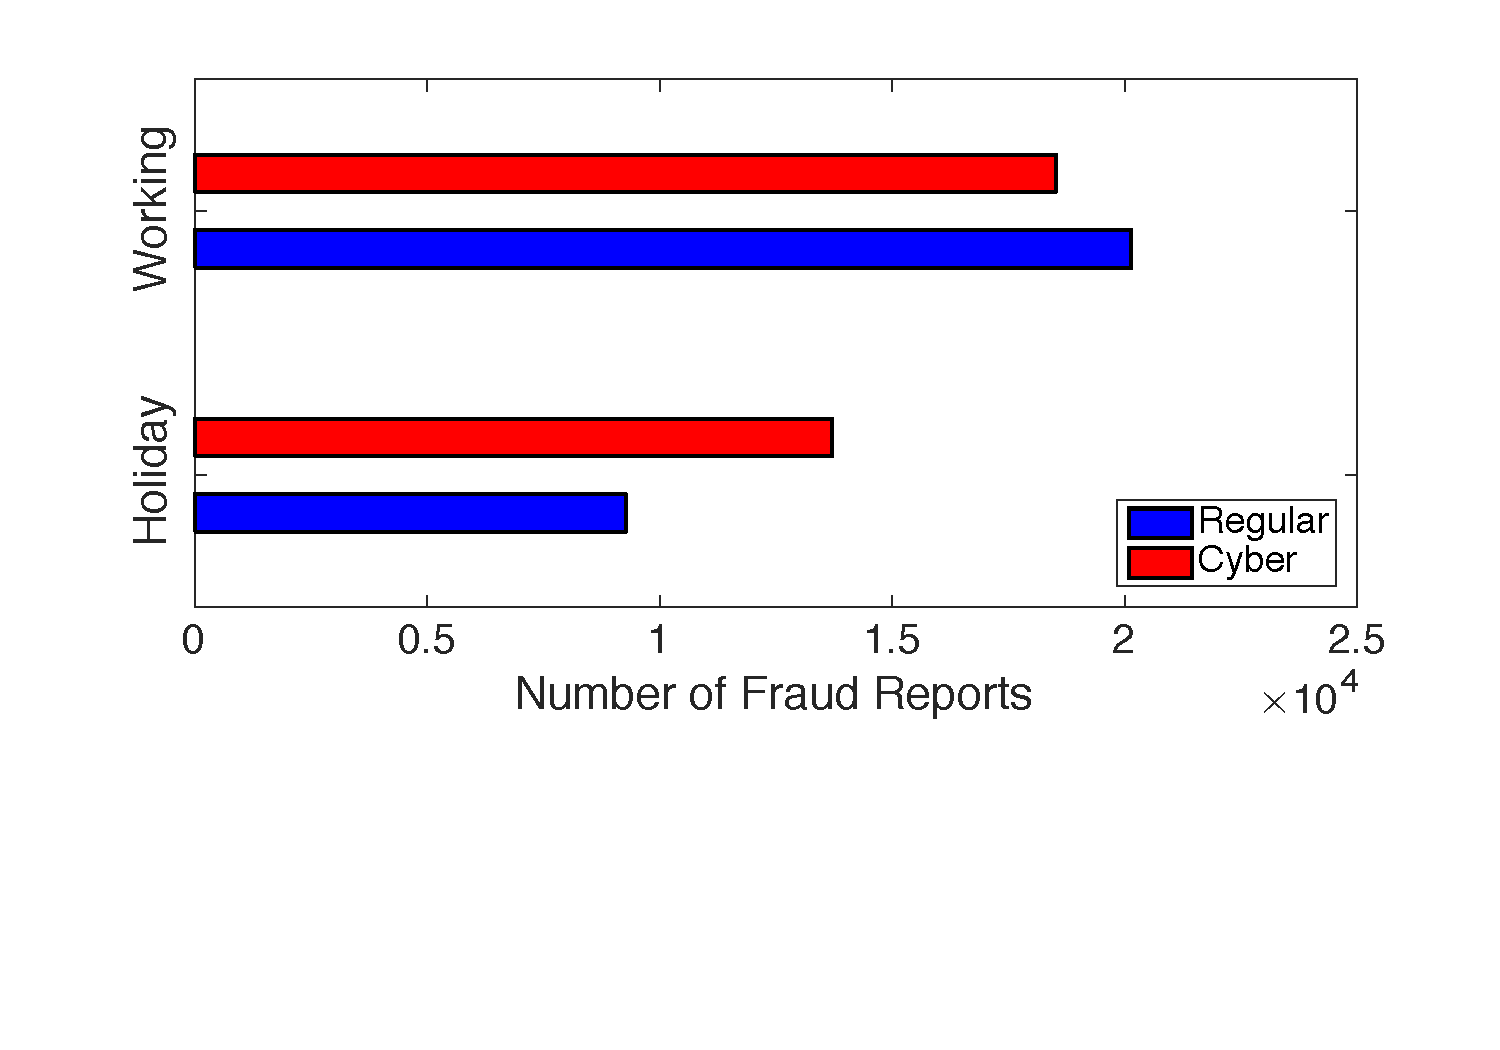
\includegraphics[scale=0.35]{graphics/reg_vs_holiday.pdf}
  \caption{Cyber and regular fraud variation during regular and holiday season}
  \label{temporal}
\end{figure}


\subsection{Fraud Reporting Methods}\label{reportingmethods}
Consumers have the ability to report complaints to the FTC via several methods and agencies. We aggregate the 26 complaint collecting entities into online and offline categories. For instance, reports made via the Internet complaint center or the FTC complaint assistant and tagged as online, while the ones issued to the FTC call center, publisher clearing house, attorney generals or other regulatory institutions are categorized and offline. Figure \ref{reportingfig} provides the distribution of how individuals opt to report cyber and regular crimes. Approximately 82\% of cyber fraud victims used an online complaint facility, and 63\% of regular fraud victims reported via offline methods.


 \begin{figure}[b]
\centering
  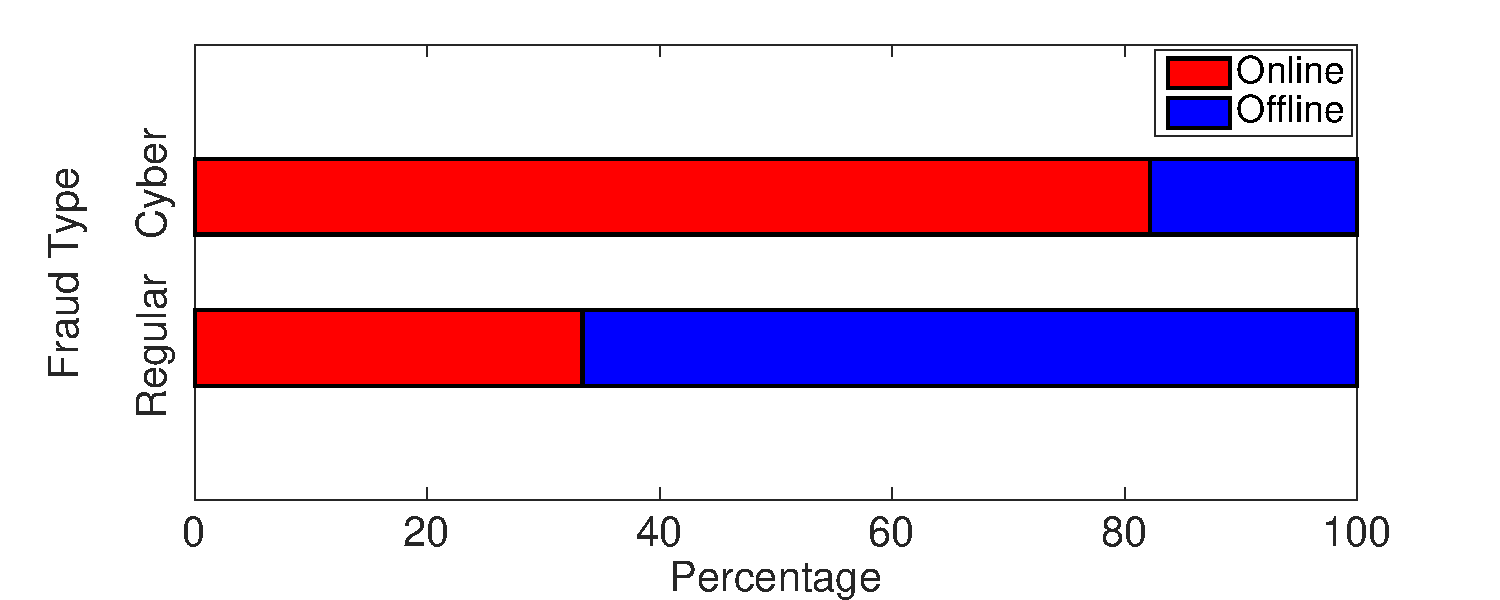
\includegraphics[scale=0.35]{graphics/reporting_methods.pdf}
  \caption{Distribution of reporting methods in for cyber and regular frauds}
  \label{cdffig}
\end{figure}

A major chunk of regular frauds are reported to offline institutions which have reduced operation during holidays. We believe this significantly contributes to the reduction bias of regular frauds value in Figure \ref{temporal}. To further validate this bias, we perform a t-test for the two fraud categories across the working and holiday time periods. The statistically significant \emph{p-value} for regular frauds in Table \ref{ttest}, rejects our null hypothesis of \emph{identical reporting trends between two the two time periods}. Additionally, we also calculate the percent increase in reporting between the last 10 holidays and 10 working days right after. While cyber reports only incase by 37\% the increase in regular fraud reports is a staggering 104\%. The ratio of increases is in line with the proportions (17:66) for offline reporting methods used by cyber and regular fraud victims. We believe that while both types of frauds experience a decrease, the decrease in cyber frauds represents a more accurate trend. These derived insights enable us to suggest more meaningful measures in section \ref{discussion} to deal with consumer fraud.

\subsection{Consumer Reaction Time}\label{fraudsters}

We evaluate how quick do the victims of a fraud report an incident. Figure \ref{cdffig} (a) shows the CDF of the number of days between the date when the fraud occurred and when in was first reported to the FTC. We do not observe any difference between the reaction time trends of cyber and regular fraud victims. The graph shows that for both fraud categories, almost 30\% of the individuals take more than a week to respond. We believe that this provides ample time window for fraudsters to maliciously act on the assets acquired from individuals. This increased delay can also be a result of individuals discovering they were victimized to a fraud at a later date that the actual incident. One example would be of a credit card theft, when the victims only realizes after they see an unauthorized transaction. Unfortunately, we do have enough information in the dataset to normalize against this trend.

\subsection{Most Common Frauds}\label{fraudsters}

Table \ref{topfrauds} provides a summary of the top frauds in each category. The significant cyber presence of impostor scams, and sweepstakes in, which have long existed in the regular fraud domain provides evidence that fraudsters are adopting new technology to execute the same frauds. We incorporate this specific insight in our discussion in section. Our results greatly match with the top sources of frauds in the FTC correlate with the frauds stated in an FTC news release in 2016 \cite{ftcpress2016}. 

\begin{table}[h]
\centering
\begin{tabular}{c|c||c|c}
\hline
\bfseries Cyber & \bfseries \% & \bfseries Regular & \bfseries \% \\
\hline
\hline
Online Shopping \& Sales & 14.1 & Impostor Fraud & 29.8\\
\hline
Impostor Fraud & 10.8 & Telemarketing & 20.1\\
\hline
Unsolicited Email & 7.71 & Debt Collection & 16.1\\
\hline
Counterfeit Check Scams	 & 7.40 & Prizes \& Sweepstakes & 15.5 \\
\hline
Prizes \& Sweepstakes & 7.40 & Grants \& Credit Loans & 4.14\\
\hline
\hline
\end{tabular}
\vspace{8pt}
\caption{Top Fraud Types}\label{topfrauds}
\vspace{-15pt}
\end{table}

\subsection{Top Fraudster Locations}\label{fraudsters}
Next, we identify the primary locations of the fraudsters within the United States and present our findings in ref{topareas}. While fraudulent entities are spread throughout, most of the heavy hitters belong to the metropolitan areas. We believe this provides an efficient disguise to the fraudulent entities.  
Numbers: 29.3\% cyber reports and 32.6\% regular reports.


\begin{table}[h]
\centering
\begin{tabular}{c|c|c}
\hline
\bfseries Metropolitan Area (MSA) & \bfseries \% Cyber & \bfseries \% Regular\\
\hline
\hline
New York, New Jersey, Long Island & 8.41 & 7.67 \\
\hline
Los Angeles, Long Beach, Santa Ana & 6.50 & 7.09 \\
\hline
Washington, Arlington, Alexandria & 4.10 & 5.78 \\
\hline
Miami-Fort Lauderdale, Pompano Beach & 4.16 & 5.40 \\
\hline
Dallas, Fort Worth, Arlington & 2.89 & 3.36\\
\hline
Chicago, Naperville Joliet & 3.17 & 3.27 \\
\hline
\end{tabular}
\vspace{8pt}
\caption{Top Metropolitan Areas Where Fraudsters are Based}\label{topareas}
\vspace{-15pt}
\end{table}

We also observe certain areas that have a high cyber to regular fraud ratio and vice versa. The San Franciso, Oakland and San Jose, Santa Clara MSAs have a cyber to regular fraud ratio of 2.21 and 5.13. The popular fraud types in these regions are Internet services, unsolicited email, and online shopping. These areas serve as a good medium for cyber fraudsters as it allows them to gel into the surrounding cyber industry. Meanwhile, The Buffalo, Niagara Falls MSA has a regular to cyber fraud ratio of 8.76 with debt collection being the significant outlier. Further investigation reveals that Buffalo has a network of debt collecteors which have responsible for multi-million frauds \cite{buffalodebt1, buffalodebt2}.


\subsection{Fraudster Coverage}\label{fraudstercoverage}

In order to understand the operational regions of fraudulent entities, we calculate the distances between consumer and fraudster zip codes. Figure \ref{reportingfig} (b) provides a cumulative distribution of the operational radii for cyber and regular fraudsters.  This analysis provides insight on weather cyber fraudsters leverage the Internet for more visibility and access to target more distant individuals. With a median distance of 993 and 861 for cyber and regular frauds, we believe that both types of fraudsters follow similar trends. This indicates that a major the Internet based communication does not provide cyber fraudsters with significant advantage over regular ones as they are able to achieve similar operational spans by using phone and mail based communication methods.

\begin{figure}[t]
\centering
  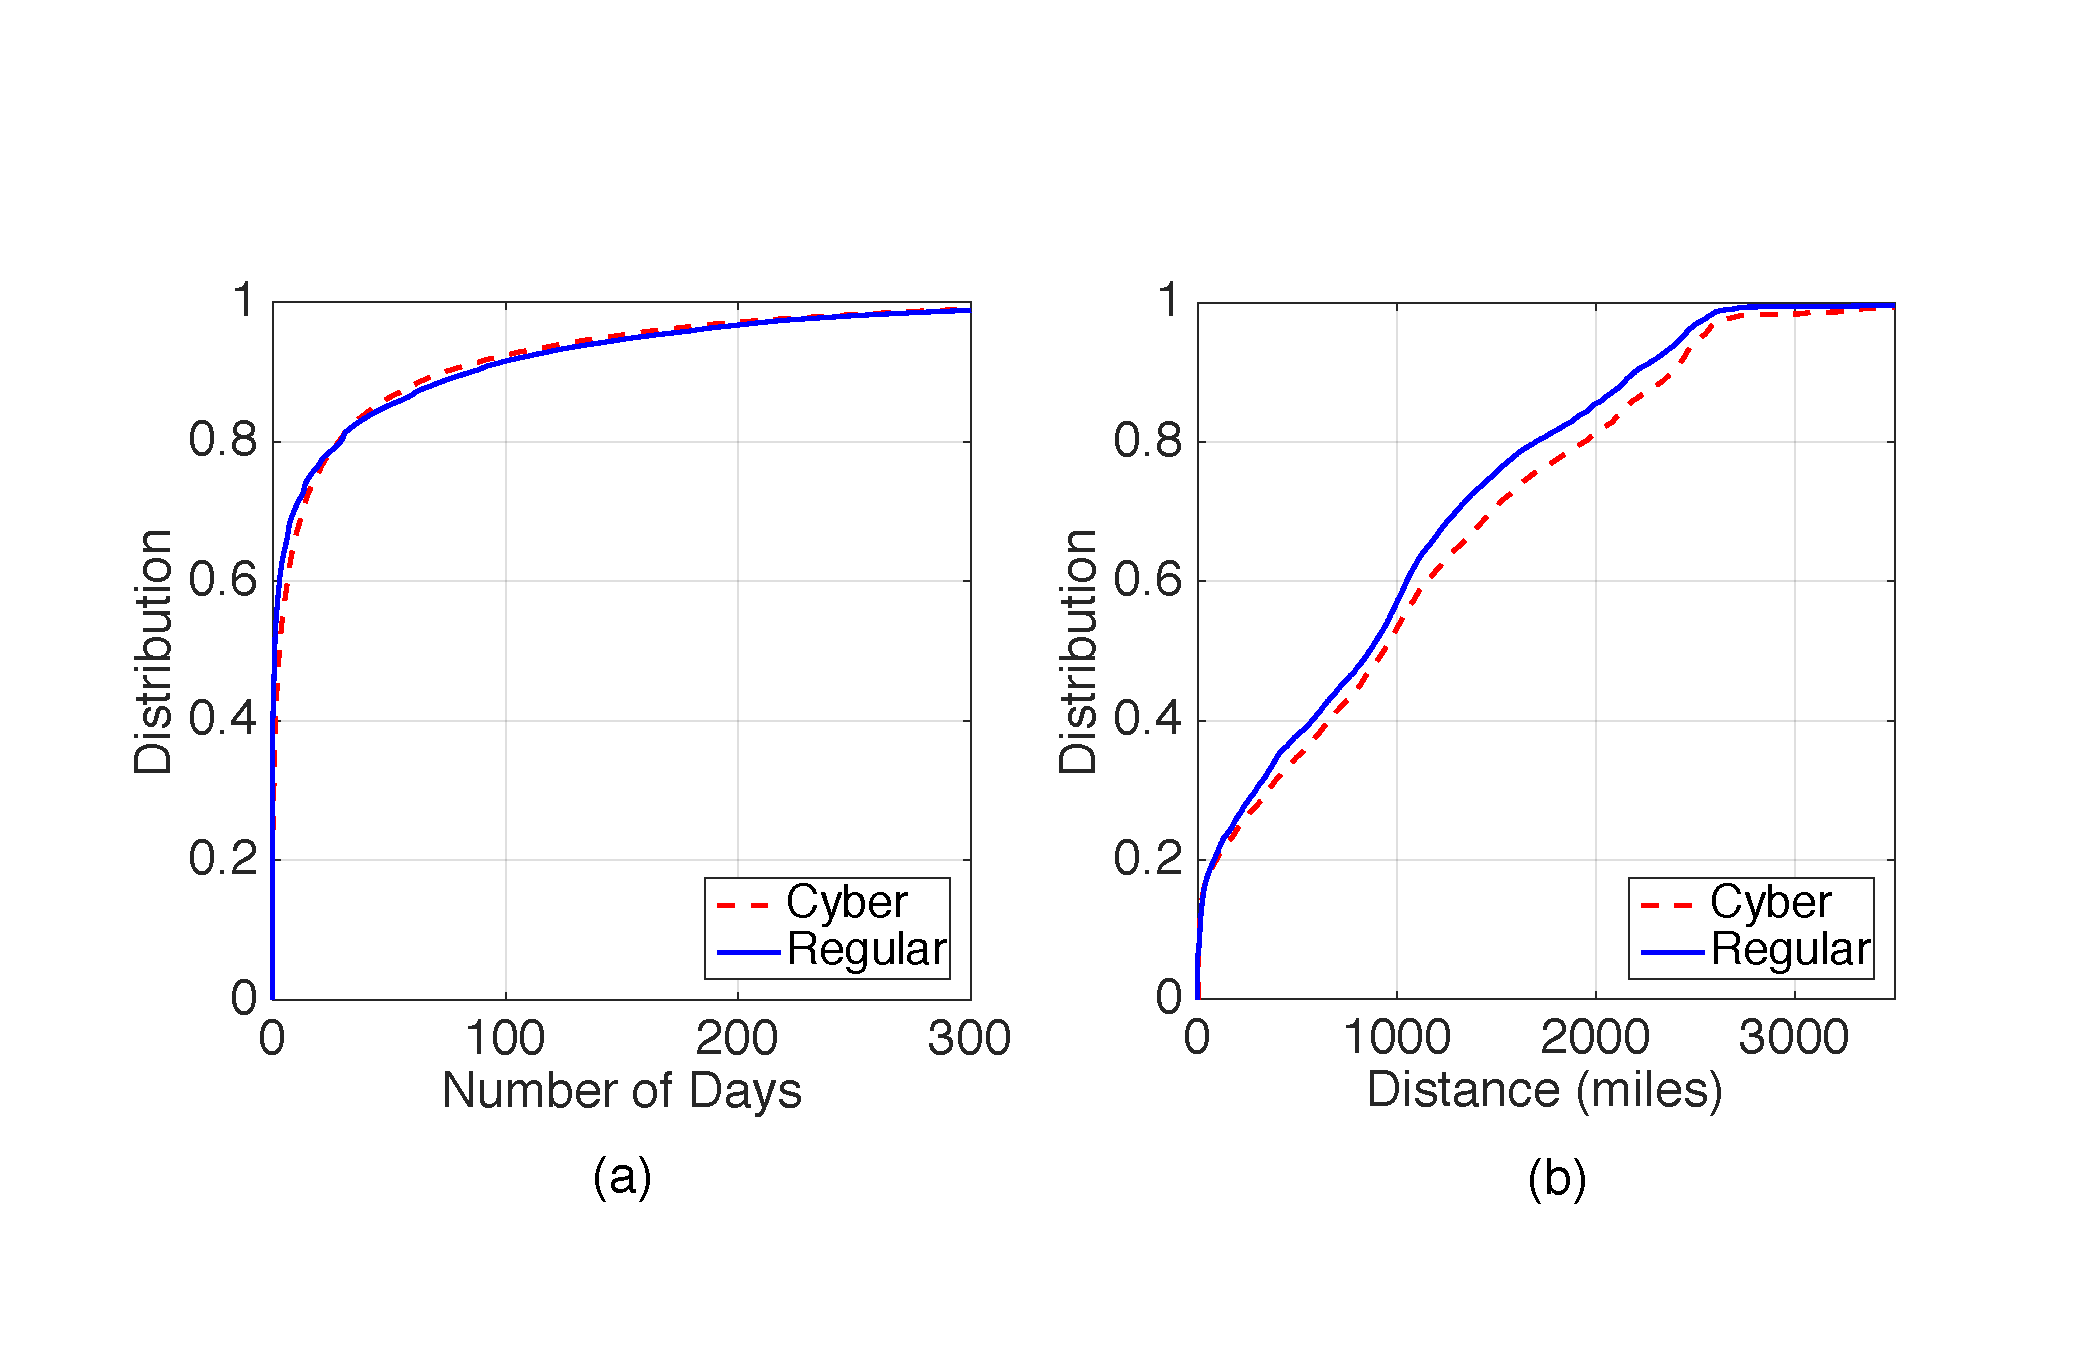
\includegraphics[scale=0.28]{graphics/dist_days.pdf}
  \caption{Distribution of reporting methods in for cyber and regular frauds}
  \label{reportingfig}
\end{figure}


\subsection{Demographic Analysis}\label{fraudsters}


\begin{table*}[h]
\noindent
\centering
\begin{tabular}{c||c|c|c||c|c|c}
\hline
\multicolumn{1}{c||}{\bfseries } & \multicolumn{3}{c||}{\bfseries Cyber Complaints} & \multicolumn{3}{c}{\bfseries Regular Complaints}\\
\hline
\bfseries Observed Variable & \bfseries Coefficient & \bfseries \emph{p-value} & \bfseries 95\% Confidence Interval & \bfseries Coefficient & \bfseries \emph{p-value} & \bfseries 95\% Confidence Interval \\
\hline
White (Non-Hispanic) & -0.0042 & 0.074 & [-0.009, 0] & -0.0013 &  0.128 & [0.003,  0]\\
\hline
Black & -0.0058 & 0.017 & [-0.011, -0.001] & 0.0017 & 0.054 & [-2.77$^{-5}$, -0.003]\\
\hline
Asian & -0.0025 & 0.468 & [-0.009, 0.004] & -0.0051 & 0.00 & [-0.008, -0.003]\\
\hline
Hispanic & -0.0026 & 0.014 & [-0.05, -0.001] & -0.0054 & 0.00 & [-0.006, -0.005]\\
\hline
Age & 0.0064 & 0.023 & [ 0.001, 0.012] & 0.0281 & 0.00 & [0.026, 0.030]\\
\hline
Income & -2.226$^{-6}$ & 8.85$^{-7}$ & [-3.96$^{-6}$ , -4.92$^{-7}$] & -3.695$^{-6}$ & 0.000  & [-4.31$^{-6}$, -3.08$^{-6}$]\\
\hline
Education & 0.0155 & 0.000 & [0.013, 0.018] & 0.0044 & 0.00 & [0.003, -0.005]\\
\hline
Unemployment & 0.0084 & 0.111 & [-0.002, 0.019] & -0.0028 & 0.138 & [-0.006, 0.001]\\
\hline
\end{tabular}

\vspace{8pt}
\caption{The description of the data fields that were primarily used in the for data calibration and analysis}\label{regressions}
\vspace{-20pt}
\end{table*}

\begin{figure}[b]
\centering
  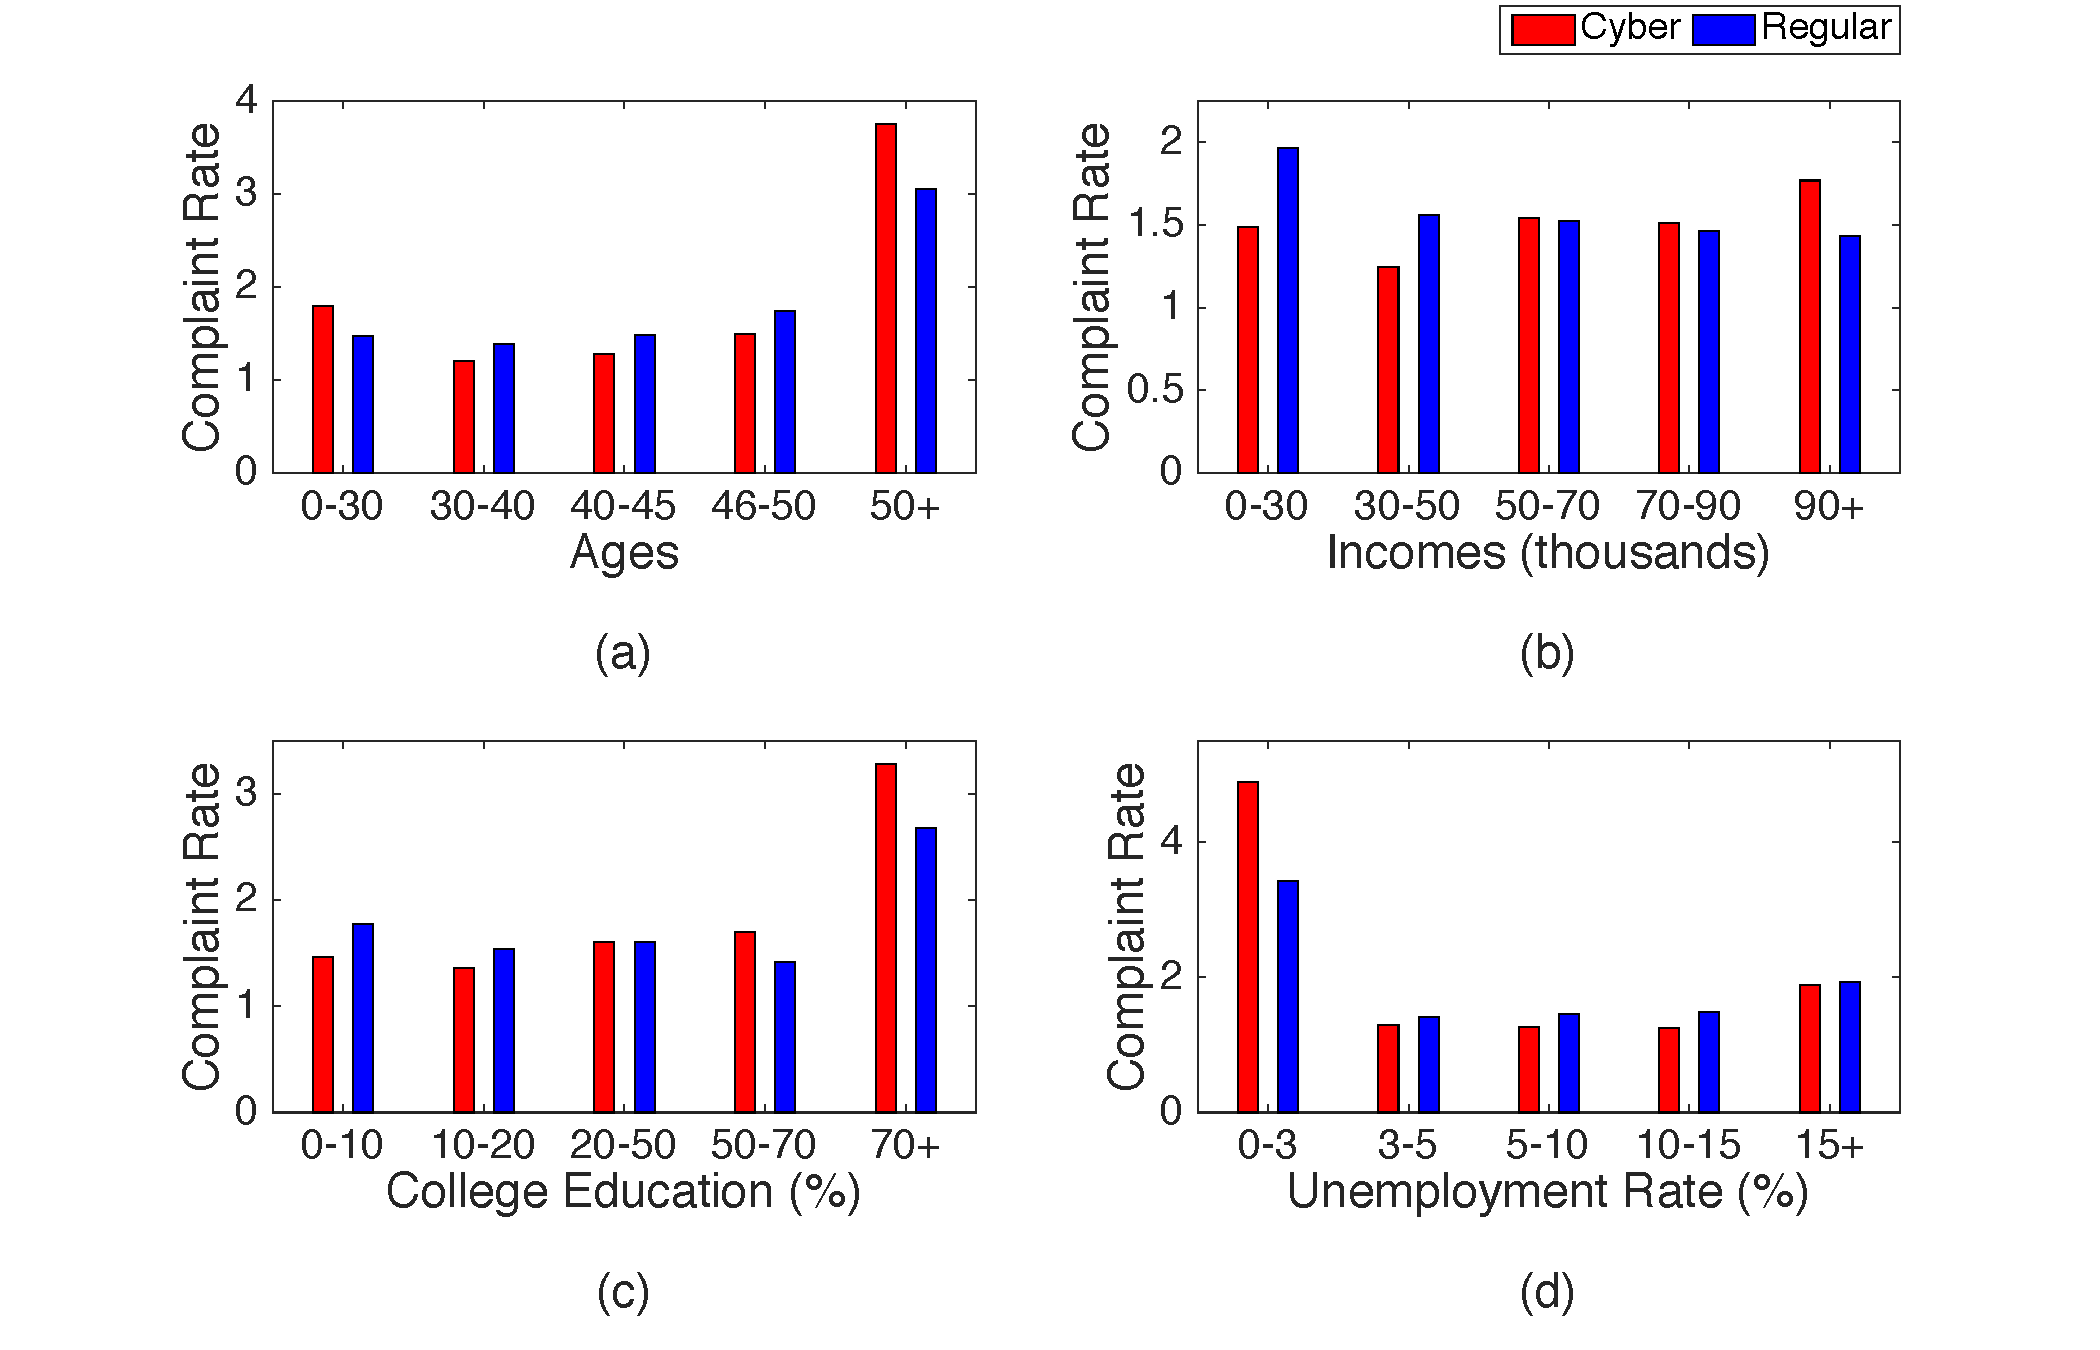
\includegraphics[scale=0.29]{graphics/demographics.pdf}
  \caption{Cyber and regular fraud trends over age, income, education and unemployment.}
  \label{demographics}
\end{figure}
To evaluate the effect of prominent demographic features we perform a logistic regression for both cyber and regular complaint rates. Table \label{regressions} summarizes our coefficients and their significance. Among ethnicities, our results generate statistically significant results for only Hispanic communities. While the coefficients suggest that frauds decrease for heavier concentrations of  Hispanics, a survey study \cite{anderson2013consumer} showed that Hispanics and Black communities are more likely to be victims of crimes. The decreasing trend is actually a result of fraud underreporting due to cultural reasons, distrust in agencies the lack of awareness and education \cite{consumerlessons}.

Other socio economic variables that we take into account are age, income, education an the rate of unemployment. In addition to the regression analysis, we investigate their variation by observing complaint rates across their distributions in Figure \ref{demographics}.

\textbf{Age:} While the differences in cyber and regular complaints remain fairly consistent, from Figure \ref{demographics} (a) we observe that individuals greater that 50 years complain significantly more than other age groups. Our significant regression values also corroborate to this trend. 


\textbf{Education:} Both cyber and regular complaints increase along with an increase in percentage education. We associate this trend with greater increased educational awareness among individuals \cite{consumerlessons}. Another subtle trend, in the increase in cyber to regular complaint ratio from 0.82 to 1.23. We associate this diverging trend to more educated individuals being active  the Internet  more frequently, and hence being more prone to online fraud{pewcollege}. Our reasoning is in line with insights from our regression analysis which additionally normalizes for other factors.

We do include income and unemployment in our analysis due to their insignificant correlation values in Table \ref{regressions}.

\section{Discussion}\label{discussion}
Based on our findings from section \ref{eval}, we elaborate some discussion points in hopes that they will assist in the development of better policies and will help prevent consumer fraud in the U.S. 

Our results indicate that while cyber frauds are on the rise, regular fraud methods still hold an equally significant share in the economy, and while policy developments are trending towards mitigating online fraud, there should be continuous awareness campaigns for phone, mail and other regular fraud types. As a result of reduced operational hours in the winter holidays, offline collection agencies experience an uneven decrease followed by a great influx of reports on resuming operation. To streamline the process, online reporting methods should be promoted.

We also learn that fraudulent entities tend to work in groups and establish networks \cite{buffalodebt2}. The fraudulent cyber establishments of San Jose and San Francisco discussed in section \ref{fraudsters}, help us understand that fraudulent entities use strategic measures to gel-in with the legitimate industry. This necessitates the need for stricter policies while registering organizations with the State agencies. Localization of fraudsters also allows inspection teams to target efficiently. 
By observing overlap between top cyber and regular frauds (Table \ref{topfrauds}) we realize that with the rise of Internet, fraudsters have their methodologies to execute scams on the Internet that were initially perpetrated through regular methods. We suggest that policy makers should work closely with technologists to devise advanced learning mechanisms similar to \cite{brause1999neural, moreau1997detection} which enables the filtering and control of fraud.

\section{Conclusion and Future Work}\label{conclusion}

The goal of this paper is to provide a comprehensive comparison of cyber and regular consumer fraud in the United States. By applying an efficient classification and measurement methodology on an FTC complaint dataset, we explore trends among cyber and regular fraud, in time, distance and location metrics as well as their variation across consumer demographics. Based on our findings, we suggest insights to aid policy development for fraud prevention. In future, we look forward to working closely with regulatory organizations and provide data driven policy insights.

\bibliographystyle{IEEEtran}

\bibliography{references} 




% that's all folks
\end{document}


